\documentclass{article}
\usepackage[brazil]{babel}

\usepackage[a4paper,top=2cm,bottom=2cm,left=3cm,right=3cm,marginparwidth=1.75cm]{geometry}
% Useful packages
\usepackage{amsmath}
\usepackage{graphicx}
\usepackage[colorlinks=true, allcolors=blue]{hyperref}
\usepackage{minted}
\usepackage{float}
\usepackage{soul}
\usepackage{booktabs}
\usepackage{graphicx}
\usepackage[table,xcdraw]{xcolor}

\usepackage{lmodern}	% Usa a fonte Latin Modern
\usepackage[utf8]{inputenc}		% Codificacao do documento (conversão automática dos acentos)




% Pacotes de citações
% ---
\usepackage[brazilian,hyperpageref]{backref}	 % Paginas com as citações na bibl
\usepackage[alf]{abntex2cite}	% Citações padrão ABNT


% First pip install pygments

% CONFIGURAÇÕES DE PACOTES
% ---

% Configurações do pacote backref
% Usado sem a opção hyperpageref de backref
\renewcommand{\backrefpagesname}{Citado na(s) página(s):~}
% Texto padrão antes do número das páginas
\renewcommand{\backref}{}
% Define os textos da citação
\renewcommand*{\backrefalt}[4]{
	\ifcase #1 %
		Nenhuma citação no texto.%
	\or
		Citado na página #2.%
	\else
		Citado #1 vezes nas páginas #2.%
	\fi}%
% --


\title{Plano de trabalho 2022}
\author{Daniel Terra Gomes}

\begin{document}
\begin{titlepage}
\begin{center}
\large
\textbf{PROGRAMA INSTITUCIONAL DE BOLSAS DE INICIA\c{C}\~{A}O CIENTIF\'{I}CA E TECNOL\'{O}GICA\\\vspace{0,5cm}
UNIVERSIDADE ESTADUAL DO NORTE FLUMINENSE DARCY RIBEIRO\\
}
\textit{Centro CCT \\
Labotat\'{o}rio LCMAT\\
\vspace{1cm}}
%Plano de trabalho para o segundo ano da bolsa }\\
\vspace{1,5cm}
\textbf{Plano de Trabalho para Renovação de Bolsa de Iniciação Científica}\\\vspace{5cm}
\end{center}
\textbf{Bolsista}: Daniel Terra Gomes\\
\textbf{Matricula}: 00119110484\\
\textbf{Orientadora}: Prof. Dra. Annabell Del Real Tamariz  \\
\textbf{Curso}: Bacharelado em Ci\^{e}ncia da Computa\c{c}\~{a}o\\
\vspace{3cm}
\begin{center}
\textbf{Titulo do Projeto}: Project-driven Data Science: Aprendendo e Mapeando\\
\textbf{T\'{\i}tulo do Plano de Trabalho}: Dirigindo para o futuro: Softwares e Algoritmos avançados que alimentam Veículos Autônomos.
%Os principais obstáculos para Veículos Autônomos no Brasil, e suas tecnologias essenciais.\\

\textbf{Fonte financiadora:} PIBICT/UENF
\end{center}
\end{titlepage}


%\maketitle
\section{Justificativa}

Os veículos autônomos (VAs) estão revolucionando o transporte e a mobilidade autônoma nos últimos anos. Esses veículos prometem aumentar a segurança nas estradas, melhorar a eficiência do tráfego, reduzir as emissões de gases de efeito estufa, aumentar acessibilidade dos cidadãos ao transporte público e privado, agilizar o transporte de encomendas e muito mais \cite{review-auto, intro-pm, mundobrasil}.

Logo, para que esses veículos atinjam todo o seu potencial revolucionário, é necessário pesquisas significativas relacionadas a questões organizacionais e tecnológicas para que os VAs atinjam o seu mais alto nível de automação, ou seja, nível 5 SAE \cite{SAE}. Visto que, como já estudado no primeiro ano de Iniciação Científica \cite{my-work-on-git}, para alcançar maior apoio organizacional e melhores níveis de automação um veículos autônomo (VA) necessita de: sensores, conexão móvel, computação de borda móvel, aprendizado de máquina, análise de dados, aprendizado distribuído e, sobretudo, aceitação do público e amparo legislativo para que essa tecnologia seja extensamente utilizada pela sociedade \cite{KPMG}, e que, também, seja capaz de, por exemplo, compreender o ambiente a sua volta e identificar o estado atual dos agentes próximos \cite{sensors-yet}.

No entanto, quando se trata de operação segura e eficiente nas estradas, é necessário ir além. Um VA não deve apenas entender o estado atual dos usuários e objetos próximos na rua, mas também antecipar proativamente o comportamento futuro, comunicar e interpretar intenções e estados dos agentes na redondeza \cite{conge}. Considerando que, uma parte considerável dessa interpretação, geralmente é prever o comportamento dos pedestres, veículos e sinalizações (ou, de um modo geral, dos usuários vulneráveis das vias) \cite{software-review}.

Essa capacidade de entendimento, interpretação  e identificação do ambiente são partes fundamentais dos componentes de um VA, sendo essas a percepção, planejamento e controle  \cite[p. ~37]{my-work-on-git}. Cujo são componentes operados e gerenciados por softwares e algoritmos que trabalham no controle do veículo a partir do seu computador central que fica encarregado de receber os dados oriundo dos diversos sensores espalhados pelo VA \cite[p. ~39]{my-work-on-git}.

    
    Em vista disso, temos como objetivo (seção \ref{objetivo}) buscar uma familiarização e compreensão do estado atual das pesquisas e projetos em detecção de ambiente, detecção de pedestres, planejamento de caminhos, e controle de movimento veicular para veículos autônomos a partir da testagem dos principais algortimos encontrados (elaborado na seção \ref{Metodologia} e \ref{etapas}). Visto que, como pesquisado e estudado no primeiro ano de projeto \cite{my-work-on-git}, fazem parte das \textit{Tecnologias Essenciais para a Direção Autônoma} e mais especificamente das \textit{Arquiteturas e Algoritmos} de VAs, cujo será a delimitação desse projeto.
 


\section{Objetivos} \label{objetivo}
Temos como objetivo desta pesquisa a familiarização e compreensão dos principais softwares e algoritmos de controle de Veículos Autônomos.



\section{Metodologia} \label{Metodologia}
Utilizaremos uma metodologia, com o propósito de revisar a literatura existente, que tem como essência desenvolver e colocar as pessoas envolvidas em contato direto com todo material já desenvolvido em relação a esta iniciação científica, que será constituída principalmente de: artigos científicos, cursos online, publicações em periódicos, jornais online, monografias, dissertações e vídeo aulas.

Nesse formato metodológico, pesquisa bibliográfica, será possível ter contato e se fundamentar com os principais materiais da atualidade relacionados a Veículos Autônomos e seus Algoritmos de Controle, de modo a ter contato com o que há de mais recente sobre o assunto.


Atrelado ao que foi apresentado, seguiremos um princípio metodológico chamado \textit{“Project-based learning”}\footnote{Aprendizagem baseada em projetos} \cite{krajcik2006project}, que visa construir soluções a partir de problemas reais em nossa sociedade. Visto que, é uma modalidade de estudo que deixa as pessoas envolvidas livres para seguir a sua curiosidade, desejo de resolver os problemas encontrados pelo caminho e de buscar por mais informações para resolvê-los. Contemplando assim os objetivos desejados para a realizar de maneira satisfatória deste projeto. 

Além disso, as pesquisas realizadas serão fundamentadas no método de pesquisa \textit{Revisão Sistemática de Literatura} (RSL) que segundo Maria Cristiane (Universidade de São Paulo) \cite{revi3}, e Davi Nakano (Universidade de São Paulo) \cite{revi2} refere-se a um tipo de investigação que se concentra em uma questão bem definida, visando identificar, selecionar, avaliar e sintetizar as evidências disponíveis relacionadas a uma questão formulada de interesse para o pesquisador.

Desse modo, amparado de todo esse ferramental teórico apresentado, seguiremos o seguinte passa a passo:



\begin{enumerate}
\item Primeiro faremos uma pesquisa e levantamento Bibliográfico de modo a agrupar e selecionar os materiais relevantes para este projeto, que será desenvolvida através dos seguintes meios na internet (Google academic, Google livros, biblioteca virtual, jornais virtuais, site das bibliotecas de universidades, plataforma CAPES, YouTube e outros). A busca nesses bancos de dados contemplará os anos de 2022 a 2023. Contudo, também, podemos fazer uso de materiais publicados há mais tempo por falta de referenciais melhores. Como palavra-chave faremos uso dos termos: Autonomous Vehicles Software, Autonomous, Cars, Mobility, Connected Car, AV, TaxiBot, Self-driving cars, Algorithmus, Deep Learning, Computer Vision, entre outros.  A pesquisa irá se limitar aos idiomas: Alemão, Inglês, Português, e podendo se estender até ao Espanhol e Francês.

\item De maneira seguinte, faremos a testagem dos algoritmos mais importantes encontrados, de modo a compreendermos os seus funcionamentos. Esses testes se limitaram aos algoritmos relacionados ao controle e autonomia dos veículos autônomos. Faremos uso de repositórios de códigos online para o armazenamento desses algoritmos, e os testes serão realizados em uma máquina local. Ressaltamos que, não nos limitaremos a linguagens de programação, e daremos prioridade a algoritmos e softwares de livre acesso.
\item Por fim, iremos elaborar o relatório final. Fazendo uso dos materias encontrados, e dos resumos e rascunhos feitos ao longo das pesquisas.
\end{enumerate}

A elaboração desse projeto terá as seguintes etapas ilustradas na Figura \ref{img_bibli}:

\begin{figure}[H]
\centering
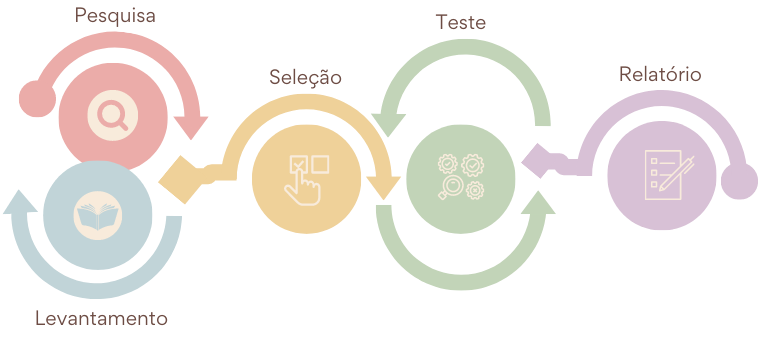
\includegraphics[width=14cm]{Figures/methodology.png}
\caption{Etapas da pesquisa Bibliográfica. Autoral.}
\label{img_bibli}
\end{figure}

\section{Etapas} \label{etapas}
A fim de alcançar os objetivos \ref{objetivo} do Projeto de Pesquisa, nesta seção do \textit{Plano de Trabalho} listamos as principais atividades que serão realizadas:


\begin{enumerate}
    \item  Pesquisa bibliográfica sobre softwares de controle para veículos autônomo;
    \item Levantamento bibliográfico algoritmos de controle de Veículos Autônomos;
    \item  Seleção dos principais algoritmos achados no levantamento bibliográfico;
    \item Teste de alguns dos principais dos algoritmos achados;
    \item Elaboração do Relatório Final.
\end{enumerate}

\section{Cronograma das atividades}
Este cronograma visa mostrar o desenvolvimento de atividades (listadas na seção \ref{etapas} e ilustada na figura \ref{img_bibli}), cada etapa \ref{etapas} foi dividida de modo a otimizar o tempo e as necessidades do projeto.

% Please add the following required packages to your document preamble:
% \usepackage{booktabs}
% \usepackage{graphicx}
% \usepackage[table,xcdraw]{xcolor}
% If you use beamer only pass "xcolor=table" option, i.e. \documentclass[xcolor=table]{beamer}
\begin{table}[H]
\centering
\resizebox{\textwidth}{!}{%
\begin{tabular}{@{}l|l|l|l|l|l|l|l|l|l|l|l|l|@{}}

\cmidrule(l){1-13}


  \multicolumn{1}{|c|}{\textbf{Etapas/Mês}} &
  \multicolumn{1}{c|}{\textbf{1º}} &
  \multicolumn{1}{c|}{\textbf{2º}} &
  \multicolumn{1}{c|}{\textbf{3º}} &
  \multicolumn{1}{c|}{\textbf{4º}} &
  \multicolumn{1}{c|}{\textbf{5º}} &
  \multicolumn{1}{c|}{\textbf{6º}} &
  \multicolumn{1}{c|}{\textbf{7º}} &
  \multicolumn{1}{c|}{\textbf{8º}} &
  \multicolumn{1}{c|}{\textbf{9º}} &
  \multicolumn{1}{c|}{\textbf{10º}} &
  \multicolumn{1}{c|}{\textbf{11º}} &
  \multicolumn{1}{c|}{\textbf{12º}} \\ \midrule

 
\multicolumn{1}{|l|}{\textbf{1}} 

\cellcolor[HTML]{A4C2F4}&
   &
  \cellcolor[HTML]{A4C2F4} &
  \cellcolor[HTML]{A4C2F4} &
   &
   &
   &
   &
   &
   &
   &
   &
   \\ \midrule
\multicolumn{1}{|l|}{\textbf{2}} &
   &
   &
  \cellcolor[HTML]{A4C2F4} &
  \cellcolor[HTML]{A4C2F4} &
  \cellcolor[HTML]{A4C2F4} &
   &
   &
   &
   &
   &
   &
   \\ \midrule
\multicolumn{1}{|l|}{\textbf{3}} &
   &
   &
   &
   &
   &
   \cellcolor[HTML]{A4C2F4}&
   \cellcolor[HTML]{A4C2F4}&
   &
   &
   &
   &
   \\ \midrule
\multicolumn{1}{|l|}{\textbf{4}} &
   &
   &
   &
&
   &
   &
   &
  \cellcolor[HTML]{A4C2F4} &
   \cellcolor[HTML]{A4C2F4}&
  \cellcolor[HTML]{A4C2F4} &
   &
   \\ \midrule
\multicolumn{1}{|l|}{\textbf{5}} &
   &
   &
  &
   &
   &
   &
   &
   \cellcolor[HTML]{A4C2F4}
   &
   \cellcolor[HTML]{A4C2F4}
   &
  \cellcolor[HTML]{A4C2F4} 
  &
  \cellcolor[HTML]{A4C2F4} 
  &
  \cellcolor[HTML]{A4C2F4} \\ 
  \bottomrule
  
\end{tabular}%
}
\caption{Etapas do plano de trabalho}
\label{tab:etapas}
\end{table}

%\centering
%\bibliographystyle{alpha}
\bibliography{bibli}
\end{document}

